\section{Test System for Cost Optimization}
To test the proposed algorithm a modified version of the feeder used in chapter \ref{A8_cahp} was used. Fig. \ref{fig:modified_feeder_2} shows the modified feeder. The only differences here are a generator is added to bus B20050P, and the energy storage added to bus B20080P to represent a microgrid at that location. The generator has a rated maximum capacity of 2000 kW. The energy storage properties are shown in Table \ref{tab:es}. Detailed descriptions about the other components of the feeder can be found in Chapter \ref{A8_cahp}, section \ref{sys}, and in Chapter \ref{CVC}, section \ref{sec:cvc_test_system}.
\begin{figure}[!ht]
\centering
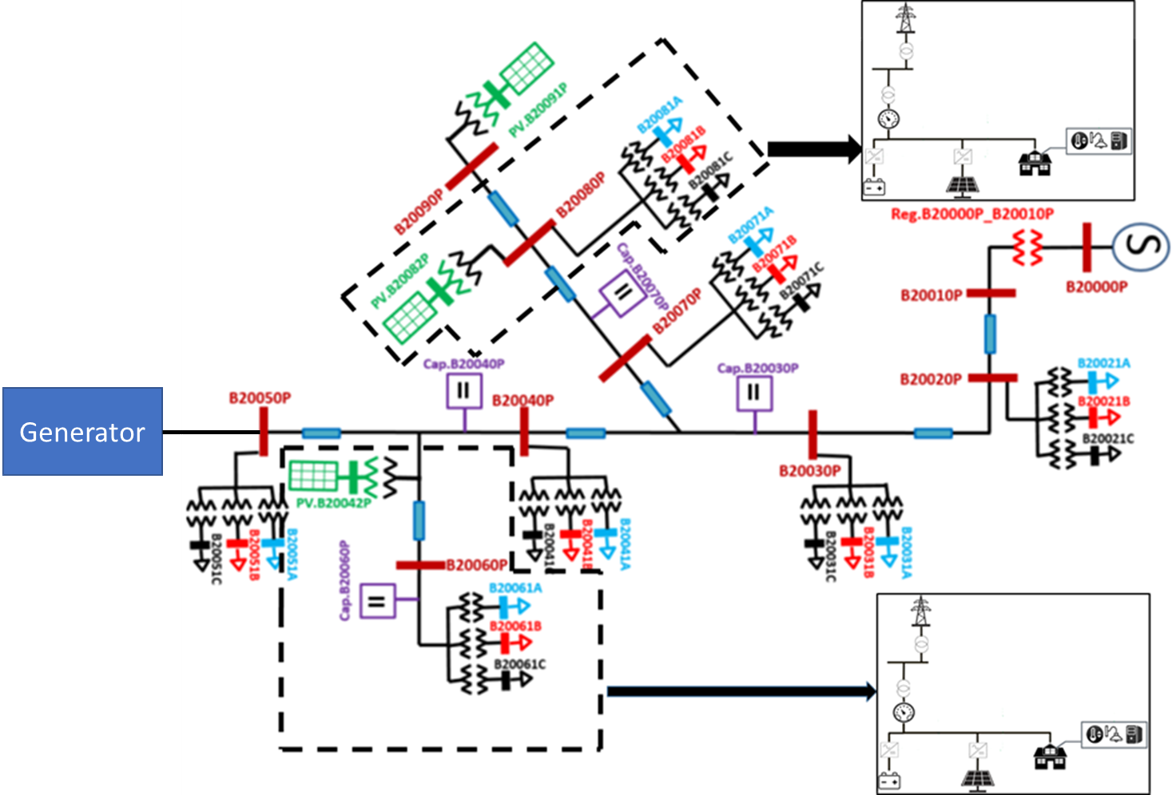
\includegraphics[width = \linewidth]{figs/A82/modified_feeder_2.png}
\caption{Distribution system used in simulation}
\label{fig:modified_feeder_2}
\end{figure}

\begin{figure}[!ht]
\centering
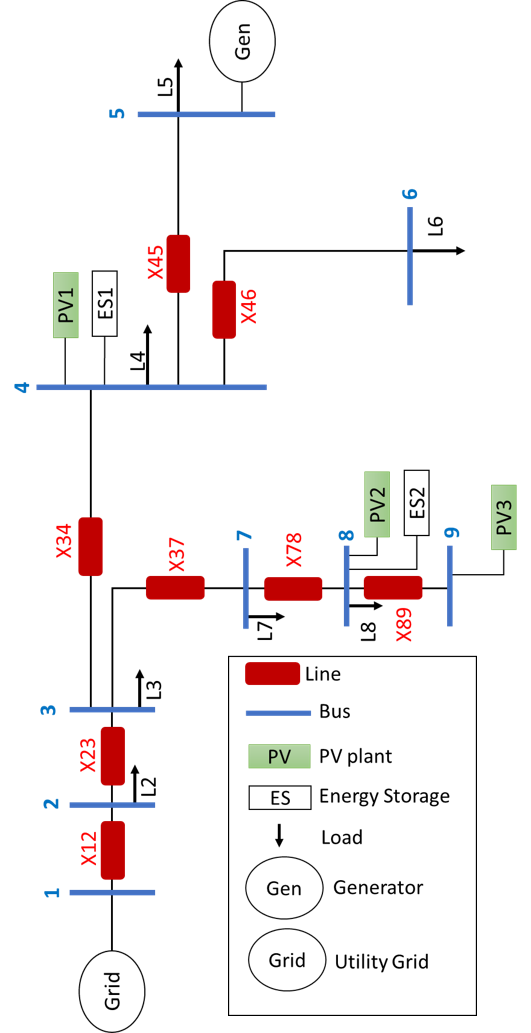
\includegraphics[width = .5\linewidth, angle = 270]{figs/A82/Grid_setup.png}
\caption{Simplified one-line diagram of the distribution system used in simulation.}
\label{fig:one_line}
\end{figure}

Fig. \ref{fig:one_line} represents a simplified one-line diagram of the feeder. Here buses 1, 2, 3, 4, 5, 6, 7, 8, and 9 represents buses B20010P, B20020P, B20030P, B20040P, B20050P, B20060P, B20070P, B20080P, and B20090P from Fig. \ref{fig:modified_feeder_2}. X12, X23, X34, X45, X46, X37, X78 and X89 are the reactance of the lines between buses 1 \& 2, 2 \& 3, 3 \& 4, 4 \& 5, 4 \& 6, 3 \& 7, 7 \& 8, and 8 \& 9 respectively. L2, L3, L4, L5, L6, L7, and L8 are the loads connected to the buses 2, 3, 4, 5, 6, 7, and 8. Pv1 \& ES1, PV2 \& ES2 are the PV \& ES connected to bus 4 and bus 8. PV3 is the PV connected to bus 9. The quadratic problem formulation for determining the edge cost according to (\ref{eq:multi_all_in1}) is as follows:\\
minimize:
\begin{multline}
\label{eq:multi_all_in1_sys}
    ( P_{grid}*rtp + |(P_{es}(1)*r_{es}(1)| + |(P_{es}(2)*r_{es}(2)| \\ + A*P_{Gen}^2 + B*P_{Gen} )*\Delta T
\end{multline}
Subject to:\\

$P_{es}(1)+P_{es}(2) = \Delta ES / \Delta T$

$(\delta_1 - \delta_2)/X_{12} = P_{Grid}$

$(\delta_2 - \delta_1)/X_{12}+ (\delta_2 - \delta_3/X_{23} = P_{L2}$

$(\delta_3 - \delta_2)/X_{23}+(\delta_3 - \delta_4)/X_{34}+(\delta_3 - \delta_7)/X_{37} = P_{L3}$

$(\delta_4 - \delta_3)/X_{34}+(\delta_4 - \delta_4)/X_{45}+(\delta_4 - \delta_6)/X_{46}=P_{L4} -$

$P_{PV1} - P_{es}(1) - P_{PV}(1)$

$(\delta_5 - \delta_4)/X_{45} = P_{L5}-P_{Gen}$

$(\delta_6 - \delta_4)/X_{46} = P_{L6}$

$(\delta_7 - \delta_3)/X_{37} + (\delta_7 - \delta_8)/X_{78}  = P_{L7}$

$(\delta_8 - \delta_7)/X_{78} + (\delta_8 - \delta_9)/X_{89}  = P_{L8} - P_{es}(2) - P_{PV}(2)$

$(\delta_9 - \delta_8)/X_{89} = -P_{PV}(3)$

$0 \leq P_{Gen} \leq \overline{P_{Gen}}$

$\underline{ES(1)} \leq ES_{current}(1)+(P_{es}(1)*\Delta T) \leq \overline{ES(1)}$

$\underline{ES(2)} \leq ES_{current}(2)+(P_{es}(2)*\Delta T) \leq \overline{ES(2)}$

$\underline{P_{ES}(1)} \leq P_{es}(1) \leq \overline{P_{ES}(1)}$

$\underline{P_{ES}(2)} \leq P_{es}(2) \leq \overline{P_{ES}(2)}$\\

The heuristic cost is calculated using (\ref{eq:multi_hu1}). The formulation of (\ref{eq:multi_hu2}) is shown in (\ref{eq:multi_all_in1_sys_hu}).\\
minimize:
\begin{multline}
\label{eq:multi_all_in1_sys_hu}
    ( P_{grid}*rtp + |(P_{es}(1)*r_{es}(1)| + |(P_{es}(2)*r_{es}(2)| \\ + A*P_{Gen}^2 + B*P_{Gen} )*\Delta T
\end{multline}
Subject to:

$(\delta_1 - \delta_2)/X_{12} = P_{Grid}$

$(\delta_2 - \delta_1)/X_{12}+ (\delta_2 - \delta_3/X_{23} = P_{L2}$

$(\delta_3 - \delta_2)/X_{23}+(\delta_3 - \delta_4)/X_{34}+(\delta_3 - \delta_7)/X_{37} = P_{L3}$

$(\delta_4 - \delta_3)/X_{34}+(\delta_4 - \delta_4)/X_{45}+(\delta_4 - \delta_6)/X_{46}=P_{L4} -$

$P_{PV1} - P_{es}(1) - P_{PV}(1)$

$(\delta_5 - \delta_4)/X_{45} = P_{L5}-P_{Gen}$

$(\delta_6 - \delta_4)/X_{46} = P_{L6}$

$(\delta_7 - \delta_3)/X_{37} + (\delta_7 - \delta_8)/X_{78}  = P_{L7}$

$(\delta_8 - \delta_7)/X_{78} + (\delta_8 - \delta_9)/X_{89}  = P_{L8} - P_{es}(2) - P_{PV}(2)$

$(\delta_9 - \delta_8)/X_{89} = -P_{PV}(3)$

$0 \leq P_{Gen} \leq \overline{P_{Gen}}$

$\underline{P_{ES}(1)} \leq P_{es}(1) \leq \overline{P_{ES}(1)}$

$\underline{P_{ES}(2)} \leq P_{es}(2) \leq \overline{P_{ES}(2)}$\\


Both (\ref{eq:multi_all_in1_sys}), and (\ref{eq:multi_all_in1_sys_hu}) are solved using the embotech ECOS solver \cite{ecos}. 